% !TeX spellcheck = hu_HU
% !TeX encoding = UTF-8
% !TeX program = xelatex
%----------------------------------------------------------------------------
\subsection{Átfogó architektúra}\label{subsec:c4:impl:arch}
%----------------------------------------------------------------------------

A C4 fordító és értelmező programok a kód nagy részében azonosak: a különbség, hogy a folyamat végén található program az LLVM által fordított bináris kimenetet generál vagy az LLVM \gls{JIT} lehetőségeit kihasználva direkt módon kezdi el kiértékelni a C4 kódnak megfelelő memóriabeli reprezentációt.

\begin{figure}[htb]
    \centerline{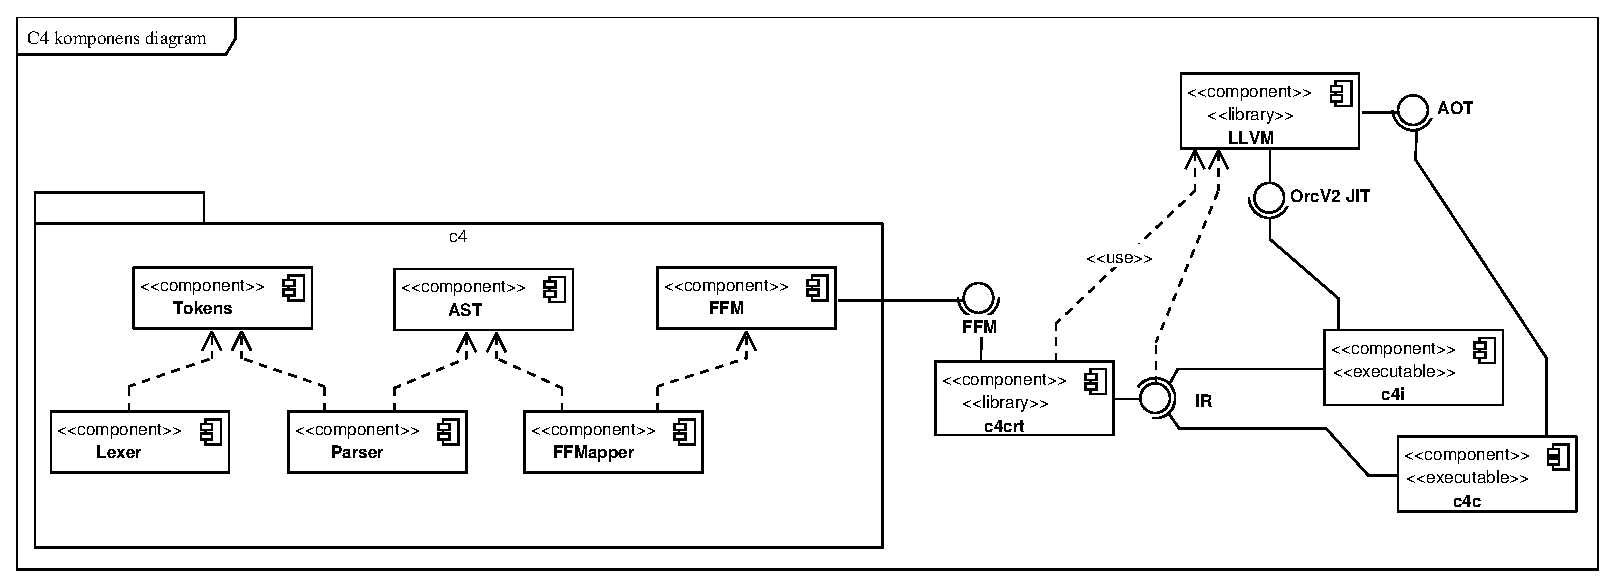
\includegraphics[width=.8\linewidth]{content/c4-comp.eps}}
    \caption{A C4 projekt átfogó ábrája}\label{fig:c4-comp}
\end{figure}

A feldolgozás az általános fordítói lépéseket tartalmazza: megjelenik a lexikális elemző (lexer), amelyik előállítja a bemenet tokenekké formált változatát és az elemző (parser), amelyik egy absztrakt szintaxis fát (\gls{AST}) állít elő.\footnote{A C4 fordítás közben nem készül külön elemzési fának (parse tree) nevezett szerkezet, amelyik minden szintaktikai elemet tárolna; a fölösleges tokenek azonnal eldobásra kerülnek.}

Az elemző lépés után azonban van egy sajátos lépés, mielőtt LLVM belső reprezentáció (\gls{IR}) készülne belőle.
Ez egy alacsony szintű, de számítógép architektúra független leírás, amelyet az LLVM biztosít.
Az említett extra lépés látszik \aref{fig:c4-comp}.~ábrán is: ez az a réteg, amelyiket egyszintű függvény-hozzárendelésnek (\gls{FFM}) hívok.
Az LLVM \gls{IR}-nak és a saját \gls{FFM}-nek részletesebb tárgyalása megtalálható \aref{sinsubsec:c4:impl:steps:ffm}.~és \aref{sinsubsec:c4:impl:steps:ir}.~szekciókban.

Az előző bekezdések tartalma mind a {\tt c4} könyvtáron belül történik meg, aminek így kimenete egy forrásfájl feldolgozásakor az előbb említett \gls{FFM} struktúrájú leírása a bemenetnek.
Ez lehetővé teszi, hogy a legbelső, általánosan csak a bementi szöveg feldolgozásával foglalkozó könyvtár az LLVM könyvtáraitól független maradjon és könnyebben és gyorsabban fordítható legyen.

A következő lépésben a {\tt c4crt} (C4 fordító futtató környezet, C4 Compiler Runtime) könyvtár felhasználja a {\tt c4} által előállított \gls{FFM} formátumú leírást, és az LLVM számára feldolgozható LLVM \gls{IR}-t elkészíti belőle.

A folyamat végén pedig vagy a {\tt c4c} vagy {\tt c4i} bináris áll, a felhasználó végcéljától függően.
Ezek az előző lépésben előállított LLVM \gls{IR}-t a megfelelő LLVM alkönyvtár számára továbbítják: a fordító binárist generál belőle, amelyet natívan lehetséges futtatni, az értelmező pedig helyben végrehajtja azt igény szerinti fordítással (\gls{JIT}).
Az optimalizálás lépése is ezekben a lépésekben történik meg, már az LLVM \gls{IR}-on.

\subsection{A C4 fordító lépései}\label{subsec:c4:impl:steps}

\subsubsection{Lexikális elemző}

A lexikális elemző elég általános, és nem tartalmaz kifejezetten érdekes megvalósításokat.
Minden token egy külön osztályba kerül, amelyik fordítási idejű konstans kifejezések (constexpr) formájában tárolják, hogy milyen literális szöveget vagy PCRE2 kompatibilis reguláris kifejezést kell hozzá illeszteni.
A megadott érték alapján dönti el a rendszer fordításkor, hogy melyiket használja hozzá.
A token által hivatkozott szöveg mindig a memóriába lapozott forrásfájl egy részére mutat, így a tokenek soha nem foglalnak extra memóriát.
A lexikai elemző osztály kérésenként egyesével egy összegtípusban (sum type, {\tt std::variant<...>}) adja vissza a mindenkori következő tokent.

\subsubsection{Elemző}

Az elemző egy kézzel írt megvalósítása a rekurzív leereszkedő elemző (recursive descent parser) algoritmusnak; kód a legtöbb helyen így ezzel megfelelően pár függvény, amelyik rekurzívan hívják egymást.
Két dolog azonban figyelmet érdemel: a függvényhívások és a felhasználó által bevezetett operátorok kezelése.

Az következők előtt megjegyzésre méltó, hogy a névfeloldás elemzés közben megtörténik, nem kell külön lépést bevezetni rá.
Ez a nyelv felépítésének következménye: minden függvény paraméterezését (paramétereinek számát, mivel dinamikus típusozás van) ismerni kell hívása előtt.
Emiatt azonban minden függvény be van jegyezve a fordító által ismert függvények közé, így mire meghívódik egyből fel is lehet oldani a megfelelő belső függvény leíró adatszerkezetre való mutatóval.

Mivel a C4 nyelv szintaxisában gyakorlatilag a szóköz a függvényhívás szintaktikája, így a függvények hívásakor egy speciális esetet kezelni kell: a hívott függvény alapján meg kell keresni, hogy mennyi paraméter tartozik hozzá és annyi darab kifejezést kell a argumentumként keresni, vagy hibát jelezni ennek hiányáról.

Az elemzőkben az operátorokat extra figyelemmel kel kezelni: a különböző precedencia szinteket és asszociativitást vagy már az elemzés közben figyelembe kell venni, vagy egy külön utófeldolgozási lépésben kell helyreállítani a megfelelő hívási sorrendet.
Emiatt elemző generátorok eszközök használatánál a különböző precedenciákat a rekurzió különböző szintjeire való elhelyezésével szokás megoldani a szabályok megadása során.
Kézzel fejlesztett megvalósítások esetén azonban egy hatékonyabb lehetőségünk is van, az \un precedencia mászó algoritmus (precedence climbing algorithm) formájában.
Az eredeti algoritmust a BCPL-ről írt könyvben definiálták BCPL-ben és szöveges formában \cite{richards_basic_1984}, de egy verziója elérhető példakóddal az ANTLR3 eszközhöz is \cite{harwell_operator_2008}.
Ennek a manuális megvalósításával hatékonyan lehetséges általánosan infix formájú operatorokat elemezni.
Annyi módosításra van szükség, hogy a konstans halmazt, amelyik a lehetséges operátorokat definiálják, egy elemzési időben változó halmazra kell cserélni.
Ezzel általános, felahasználó által definiált asszociativitású és precedenciájú operátorokat lehetséges helyesen \gls{AST}-be konvertálni.
Ennek a folyamatnak a ki és bemenetét mutatja be \aref{fig:c4-ast}.~ábra.
Ezen az ábrán a {\tt ->}, {\tt @} és {\tt \#} után álló mutatók értékei egyszerűsítve lettek a {\tt c4c} \gls{AST}-t lekérdező kimenetében, hogy könnyebben olvasható legyen az ábra.

\begin{figure}
    \centerline{
\includegraphics[width=.7\linewidth]{figures/ast.pdf}}
    \caption{A C4 forrásból készített AST (mutató értékek egyszerűsítve)}\label{fig:c4-ast}
\end{figure}

\subsubsection{Egyszintű függvény-hozzárendelő}\label{sinsubsec:c4:impl:steps:ffm}

A következő lépés az egyszintű függvény hozzárendelés.
Ez egy olyan köztes lépés, amelyik a megvalósítást teszi könnyebbé.
A következő lépés kimenete (LLVM \gls{IR}), és ennek a lépésnek a bemenete (\gls{AST}) között akkora különbség van szemantikailag, hogy a megvalósító kód olvashatóságának és karbantarthatóságának rovására menne rögtön egy lépésben
Ez az eltérés könnyen látszik: az \gls{AST}-ben leírt nyelv egy lusta kiértékelésű, dinamikusan típusos, immutábilis nyelv, LLVM \gls{IR} pedig regiszterek szintjén működő, gép független assembler nyelv.

Az \gls{FFM} réteg ezt a problémát egyszerűen úgy oldja meg, hogy sok implicit dolgot, ami az eredeti C4 nyelvben és így az \gls{AST}-ben sem jelenik meg külön, azt egy külön \gls{FFM} szintű nyelvi elembe emeli ki.
Kiemelkedő a függvényhívások két fajtája: a blokk legfelső szintjén azok, amelyek direkt a kapcsos zárójelek között vannak, átlagos szorgos kiértékeléssel futnak le, így ezeket egyszerű {\tt call} elemekbe kell átfordítani; minden más legfelső függvény argumentumaként átadott függvényhívásból viszont lustán kiértékelt verziót.
Utóbbira az \gls{FFM} szinten a {\tt pack} hívással vannak megjelölve, amelyik későbbi lépésben generált segédfüggvényeiben is megjelenik, amelyek a {\tt c4rt\_package\_t} típust használják egy-egy ilyen függvényhívás támogatására.

Az \gls{FFM} névadó lépéséről még nem esett szó.
Minden blokk a C4 nyelvi szinten egy saját függvényként viselkedik: vannak paraméterei, van valamekkora törzse amelyik kiértékelésekor visszaad valamilyen értéket.
Viszont a fordítás végére a bemenetből egy LLVM \gls{IR} formátumú kimenetet kell előállítani, amelyik nem támogat egymásba ágyazott függvény definíciókat.
Így az összes valamilyen módon felépített blokk egymásba ágyazást fel kell oldani, és a legfelső egy szintre kell hozni.

Ehhez szükség van valamilyen névátalakítás (mangling) műveletre, hiszen minden ilyen blokknak a programon belül globálisan egyedi nevet kell adni, az anonim blokkok és blokkokon belül definiált függvények miatt viszont ez nem teljesül automatikusan.
Ennek a konkrét részleteire most nem térek ki, mert nem kifejezetten érdekes.
A lényegi lépések nagy vonalakban, hogy minden anonim blokk a direkt beágyazó blokkbeli sorszámát kapja meg névnek, és a generált teljes névben a blokk saját nevét megelőzi minden ősének a neve beágyazási sorrendben.
Megjegyzendő, hogy az operátorokat is itt alakítom át egyszerű csak az angol ábécé karaktereit tartalmazó függvénynevekre, az operátorok {\tt \_Co}-val, az egyszerű szimbólumok {\tt \_Cs}-el kezdődnek, így a {\tt +} operátor és a {\tt p} nevű függvény nem okoznak névütközést.

Adódik még egy probléma az egyszintű függvények létrehozásával.
Egy blokkon belül definiált blokk C4-ben egyszerűen, extra jelölés nélkül tud hivatkozni a külső függvényekre vagy paraméterekre.
De ha minden függvényt egy globális szintre kell hozni, akkor ezeket az implicit hivatkozásokat a függvények törzsében fel kell oldani egy érvényes memóriacímből való olvasásra.
Azokat a függvényeket, amelyeket ilyen módon át kell alakítani lezárásnak (closure, és innentől az angol nevét használom) hívjuk.
Speciális tulajdonságuk, hogy a viselkedésük függővé válik a létrejöttük pillanatában látható változók értékeitől.
Ezt mutatja be \aref{fig:closure-bhv}.~ábrán található kódrészlet: a closure viselkedése megváltozik az {\tt a} paraméter értékétől.

\begin{figure}[htb]
    \begin{lstlisting}[gobble=8]
        let mk_closure { |a|
            { a + 1 } # <- ez a blokk a closure
        }

        # &(...)/N egy kifezejzében értékként tárolt függvény hívása
        println &(mk_closure 40)/0 # => 41
        println &(mk_closure 41)/0 # => 42
    \end{lstlisting}
    \caption{A closure viselkedés bemutatása}\label{fig:closure-bhv}
\end{figure}

Az utolsó megoldandó probléma az a belépési pontja a programnak.
A C és hozzá hasonló nyelvekben a program futásának kezdete egy függvény formájában van definiálva például C-ben ezt a szerepet a globális {\tt main} függvény tölti be.
Vannak nyelvek azonban, mint \pl Python és Ruby, amelyek ezt nem definiálják, hanem a programként adott fájl sorban kezd el futni, külön belépési függvény nélkül.
Ezek általában a rugalmasabb, dinamikusan típusos nyelvekre jellemző, és a C4 is ebbe a kategóriába tartozik.
Az LLVM \gls{IR} azonban a belépési függvény definíciójánál alacsonyabb szintű.
A program futásának kezdetét az operációs rendszer által meghatározott módon kell kezelni.
C nyelv és a fordítók ezt az operációs rendszer függő megvalósítást a megfelelő rendszerhez tartozó C könyvtárban.
Ezzel párhuzamosan egy hasonló megvalósítást adok a C4 fordítás esetében is: az a kód, amelyik nem tartozik semmilyen függvényhez, az az \gls{FFM} rétegben egy {\tt \_C@main} függvény törzsébe kerül generálásra.
A bináris generálásnál pedig a platformnak megfelelő módon meghívja ezt a függvényt.
A ,,@'' szimbólum garantálja, hogy nem lesz névütközés C4-ben definiált függvényekkel, LLVM pedig tudja kezelni ezt a nem szokványos azonosító nevet.

Ezeket a lépéseket és megoldásokat használva előáll az \gls{FFM} réteg végén egy \gls{FFM} formátumú leírása a bemeneti C4 forrásból előállított \gls{AST}-nek.
Ennek a transzformáció eredménye \aref{fig:c4-ffm}.~ábrán látható.
Ezen az ábrán nagyszerűen látszik az is, hogy a C4 a függvényeket és operátorokat teljesen egyformán kezeli a elemzési lépés után.

\begin{figure}[htb]
    \centerline{
\includegraphics[width=.7\linewidth]{figures/ffm.pdf}}
    \caption{A C4 forrásból készített FFM}\label{fig:c4-ffm}
\end{figure}

\subsubsection{\gls{IR} előállítása és kimenet generálása}\label{sinsubsec:c4:impl:steps:ir}

Az utolsó lépésben kerül előállításra az előzőekben már említett LLVM \gls{IR} leírása az eredeti C4 kódnak.
Ez egy olyan formátuma az LLVM rendszernek, amelyiket bemenetként várnak a különböző alrendszerek.
Ez szolgál egy olyan rétegként, amelyik elég általános ahhoz, hogy ne kötődjön egy konkrét hardverhez sem túlságosan, de elég alacsony szintű ahhoz, hogy a lehető legtöbb olyan koncepciót, amivel egy-egy platform assembly nyelve rendelkezik képes kifejezni.

Az LLVM \gls{IR} egy úgy nevezett statikus egyszeri értékadás (\gls{SSA}) formát használ, amelyikben minden regiszter pontosan egyszer állhat értékadás bal oldalán.
(A regiszterek száma nem korlátozott.)
Az ennek a feltételnek megfelelő utasítások sorát pedig egy-egy felbonthatatlan egységként\footnote{Félreértéseket elkerülendő, a párhuzamosítási kontextusban is használt ,,atomi'' kifejezés használatát kerülöm. Párhuzamos kiértékelés esetén egy egyszerű blokk lefutása nem garantáltan atomi, de az még akkor is garantált, hogy ha belépünk egybe, akkor annak minden utasítását végrehajtjuk.} lefutó egyszerű blokkba (basic block) kell rendezni, amelyek között (feltételes) ugrásokkal lehet váltani a blokk végén.
Ha ezeket a blokkokat felrajzoljuk egy gráf csúcsainak, majd az ugrások irányával azonos irányba behúzunk éleket, akkor egy \un vezérlésfolyamgráfot (\gls{CFG}) kapunk, amivel a függvények teljes törzsét írjuk le.
Egy ilyen \gls{SSA} transzformációra látható egy egyszerű példa \aref{fig:ssa-tr}.~ábrán.

\begin{figure}[htb]
    \centering
    \begin{subfigure}{.2\linewidth}
        \begin{lstlisting}[gobble=12,numbers=left]
            a = 1
            if c > 0
              a = 2
            print a
        \end{lstlisting}
        \caption{Pszeudokód}
    \end{subfigure}
    \begin{subfigure}{.6\linewidth}
        \centerline{
\includegraphics[width=.95\linewidth]{figures/ssa.pdf}}
        \caption{\gls{SSA} átírás egyszerű blokkokkal egy \gls{CFG}-be}
    \end{subfigure}
    \caption{Pszeudokód példa átírása \gls{SSA} formába}\label{fig:ssa-tr}
\end{figure}

Ennek a sémának az előnye az fordításkor használt optimalizáló és a hozzá fejlesztett egyes optimalizációs lépések megvalósításában jelenik meg, ami miatt ezek sokkal könnyebben kivitelezhetőek, mert minden regiszter értéke egyértelműen ismert az egyetlen értékadásból, amelyikben bal oldalt szerepel.
Ez alapján pedig könnyebben lehet különféle következtetéseket levonni, információt gyűjteni a kód viselkedéséről, ami alapján pedig a kód formáját átírni, hogy az jobban közelítse az optimálisat.
Mivel ez a séma nagyon elterjedt a fordító backendekben, az optimalizációs lépésekből létezik számos akadémiai -- például a $\phi$ függvények hatékonyabb elhelyezésével foglalkozók \cite{boissinot_revisiting_2008} -- de a gyakorlatban megvalósítottból is megannyi implementáció létezik például az LLVM kódbázisában a saját \gls{IR} formátumán készen futtatható módon.

Összességében, az LLVM használatához át kell alakítani a bemeneti forrásnyelv leírását \gls{SSA} formába.
Erre a feladatra már a kilencvenes éveke eleje óta létezik algoritmus \cite{cytron_efficiently_1991} és annak különféle javításai \cite{briggs_practical_1998}.
Röviden kifejtve azonban az \gls{IR} generálásának szempontjából két nagy következménye van.
Első, hogy ha egy forrásnyelvi változó többször kap értéket egy program folyama során, akkor azt olyan módon kell \gls{SSA} formába hozni, hogy minden értékadásnál egy új verziót kell hozzá bevezetni egy regiszter formájában.
A \gls{CFG} és érintett $\phi$ függvények szerinti jelenleg megfelelő verziót pedig számon kell tartani, és a változóra vonatkozó hivatkozásokat erre a legutolsó regiszter példányként kell generálni.
A másik, hogy az elágazó \gls{CFG} esetén a $\phi$ függvényeket megfelelő paraméterezéssel le kell generálni minden blokk elejére, amelyikbe több beérkező él is van.

A teljes problémakört azért fejtettem ki, mert a C4 megvalósításban az általános algoritmusnál egyszerűbb megoldást lehetséges adni.
Az első következmény nem játszik szerepet, hiszen minden immutábilis a forrásnyelvben is, így nem kell ezzel külön foglalkozni, automatikusan megfelel az \gls{SSA} elvárásainak.
De ami érdekesebb, hogy a másodikkal sem kell foglalkozni, mert nincs külön elágazás vagy ciklus eleme a nyelvnek, ami nehézségeket okozna az {\tt if/3} például is csak egy olyan függvény, mint \aref{fig:c4-ffm}.~ábrán definiált {\tt add/2}.
Meghívása pedig emiatt teljesen azonos, és így nincs elágazás.
Ezeknek megfelelően az \gls{IR} generálásánál csak az egyes struktúrákba való indexelést (lusta paraméterátadás struktúráinál) és a lusta függvényhívást kell legenerálni a primitívebb ekvivalenseikbe.
Ezek már nem kifejezetten nehéz feladatok, mivel segédfüggvényként lehetséges bevonni olyan kódrészleteket, amelyeket már előre és egyszer megvalósítottam, kézzel.
A segédfüggvények feladatköre \aref{sec:c4:rt}.~szekcióban tárgyalt viselkedések megvalósítása.

Kérdéses lehet az előző bekezdésben adott azon állítás, hogy nincs elágazás generálása szükség: ha egyáltalán nincs elágazás, akkor hogyan lehetséges megvalósítani azt, hogy a nyelvben mégis elérhető és használható az {\tt if/3} függvény?
A C4 képes arra, hogy olyan módon definiáljon igaz és hamis értékeket, majd ezek felett egy elágazás szerkezetet, hogy az a más nyelvekből megszokott szintaktikájú és szemantikájú {\tt if} szerkezetre hasonlítson.
Ez a megadása az értékeknek megfelel a $\lambda$-kalkulusban definiált Church-boolean \cite[2.4.2.~szekció]{kemp_theoretical_2007} koncepciónak, amivel a logikai értékeket és olyan logikai függvényeket, mint az ÉS és a VAGY lehet megvalósítani $\lambda$-kalkulusban.
Az így megadható függvények közé tartozik egy olyan elágazás is, amelyik az első bemenetének értéke alapján vagy második vagy a harmadik bementét adja vissza értékül.
Ez pontosan az az if konstrukció, amelyiket függvényként lehet használni, többek között C4-ben is.
Ennek a megadása látható \aref{fig:churh-bools}.~ábrán, ahol az ekvivalens C4 kóddal együtt szerepel.

\begin{figure}[htb]
    \begin{subfigure}{.45\linewidth}
        \begin{align*}
            \mathrm{true}  &\triangleq (\lambda tf.t) \\
            \mathrm{false} &\triangleq (\lambda tf.f) \\
            \mathrm{if}    &\triangleq (\lambda ctf.c\;t\;f) \\
            \mathrm{if}\ \mathrm{true}&\;\mathrm{false}\;\mathrm{true} \overset{\beta}{\rightsquigarrow}  \mathrm{false}
        \end{align*}
    \end{subfigure}
    \begin{subfigure}{.45\linewidth}
        \begin{lstlisting}[gobble=12,numbers=left]
            # Hogy elkerüljem a beépített függvényekkel
            # való névütközést c-vel vannak prefixelve
            let ctrue { { |t f| &(t)/0 } }
            let cfalse { { |t f| &(f)/0 } }
            let cif/3 { |c t f| &(c)/2 t f }

            cif ctrue
                println "true"
                println "false" # => true
        \end{lstlisting}
    \end{subfigure}
    \caption{A Church-booleanok $\lambda$-kalkulusban és C4-ben}\label{fig:churh-bools}
\end{figure}

A tényleges megvalósítás azonban mégsem ezt a megoldást használja, mivel így minden elágazás esetén két indirekt címre való ugrást kell végezni végrehajtás közben.
Egyet, amikor a beérkező feltétel paraméterben lévő blokkot értékeljük ki, majd amikor ez a blokk továbbugrik a szintén paraméterében kapott igaz vagy hamis blokkot reprezentáló értékre.
Ellenben, ha ezt direkt módon LLVM \gls{IR}-ben adom meg, akkor egy indirekt függvény címére kell csak ugrani: a megfelelő igaz vagy hamis blokkéra.
A logikai érték kiértékelését egy egyszerű szám összehasonlítással meg lehet valósítani.
Erről \aref{ssubsec:c4:rt:types:nan}.~részben leírtak alapján van könnyedén lehetőség.













